\documentclass[a4paper, adobefonts]{ctexart}

\usepackage[top=1.2in, bottom=1.2in, left=1in, right=1in]{geometry}
\usepackage{minted, graphicx, hyperref}

\hypersetup{colorlinks=true, linkcolor=blue}

\title{操作系统实验报告9}
\author{蔡日骏\quad12348003}

\begin{document}
\maketitle

\section{简介}
本次实验为AssignmentOS添加文件系统支持,包括一个简单的软盘控制器驱动程序和FAT12文件系统
驱动程序,以及一个对底层文件操作进行封装虚拟文件系统层。此外,为了支持应用程序的加载运行,
内核中添加了多个系统调用的支持。

\section{实现}
\subsection{软盘控制器驱动程序}
AssignmentOS中实现的软盘控制器驱动程序非常简单,只实现了读取功能,且没有足够的错误恢复机制,
但是足以用作演示。

简单来说,此驱动程序对软盘控制器进行操作,并通过DMA\footnote{ISA DMA}进行数据访问。在进行DMA传输
等不需要CPU参与操作时,驱动程序会自动挂起当前进程,内核的任务调度器会把控制器交给其他进程。

驱动程序的主要代码如下。

\begin{minted}{c}
/* 初始化软盘控制器 */
bool init_fdc()
{
    int i;
    uint8_t tmp;
    IDT[0x26] = make_int_desc(0x8, (uint32_t)inthandler26);
    enable_irq(6);
    fdc_reset = false;
    outb(DATARATE_SELECT_REGISTER, 0x80); /* 重置软盘控制器 */
    while(!fdc_reset)                     /* 等待IRQ6,但调度器未初始化只能挂起 */
        hlt();
    for(i = 0; i < 4; ++i) {
        fdc_send_byte(SENSE_INTERRUPT);
        fdc_get_byte(&tmp);
        fdc_get_byte(&tmp);
    }
    outb(CONFIGURATION_CONTROL_REGISTER, 0); /* 设置数据传输速率 */
    fdc_send_byte(SPECIFY);                  /* 设置软盘控制器工作参数 */
    fdc_send_byte(0xCF);
    fdc_send_byte(0x6);
    outb(DIGITAL_OUTPUT_REGISTER, 0x1C);     /* 启动马达 */
    return true;
}

/* 移动磁头到指定的磁道 */
bool fdc_seek(uint8_t cyliner)
{
    bool result = true;
    uint8_t tmp;
    cli();
    fdc_send_byte(SEEK);
    fdc_send_byte(0);
    fdc_send_byte(cyliner);
    wait_event(WAIT_IRQ6);   /* 等待IRQ6,此时调度器已初始化,可以进程切换 */
    fdc_send_byte(SENSE_INTERRUPT);
    fdc_get_byte(&tmp);
    if(tmp & 0xC0)
        result = false;
    fdc_get_byte(&tmp);
    sti();
    return result;
}

/* 设置ISA DMA控制器 */
bool fdc_DMA_init(bool write, void *addr, size_t len)
{
    if((uint32_t)addr > 0xFFFFFF) /* ISA DMA只能在物理内存前16M上操作 */
        return false;
    if(len > (1 << 16))
        return false;
    --len;
    cli();
    outb(0x0A, 0x6);
    outb(0x0C, 0);
    outb(0x0B, write ? 0x4A : 0x46);
    outb(0x04, ((uint32_t)addr) & 0xFF);
    outb(0x04, (((uint32_t)addr) & 0xFF00) >> 8);
    outb(0x81, (((uint32_t)addr) & 0xFF0000) >> 16);
    outb(0x05, len & 0xFF);
    outb(0x05, len >> 8);
    outb(0x0A, 0x2);
    sti();
    return true;
}

/* 读数据到内存 */
bool fdc_read(int cyliner, int head, int sector, int nsect, void *target)
{
    bool result = true;
    uint8_t tmp;
    if(!fdc_DMA_init(false, target, 512 * nsect)) /* 设置DMA */
        return false;
    cli();
    fdc_send_byte(READ_DATA | 0xC0);
    fdc_send_byte(head << 2);
    fdc_send_byte(cyliner);
    fdc_send_byte(head);
    fdc_send_byte(sector);
    fdc_send_byte(2);
    fdc_send_byte(18);
    fdc_send_byte(0x1B);
    fdc_send_byte(0xFF);
    wait_event(WAIT_IRQ6);  /* 挂起当前进程,等待缓慢的IO操作完成 */
    fdc_get_byte(&tmp);
    if(tmp & 0xC0)
        result = false;
    fdc_get_byte(&tmp);
    fdc_get_byte(&tmp);
    fdc_get_byte(&tmp);
    fdc_get_byte(&tmp);
    fdc_get_byte(&tmp);
    fdc_get_byte(&tmp);
    sti();
    return result;
}
\end{minted}

\subsection{文件系统}
AssignmentOS从设计上支持多种不同的文件系统格式\footnote{虽然目前只实现了FAT12},为了统一文件访问的
操作,内核中实现了一个简易的类似虚拟文件系统的层次对下层的操作进行封装。

下面先介绍AssignmentOS对FAT12文件系统的实现。

由于AssignmentOS在为进程分配进程任务控制块所需的内存空间时会进行页对齐,因此实际上每个进程都会有一段
多余的空间。在实现文件系统时,由于这部分多余空间正好能够保证在物理内存的前16M内,因此可以被利用起来
作为IO缓冲区以减少IO次数,极大地提升性能。

下面的函数会检查当前进程的IO缓冲区中数据是否所需,如果是则直接返回,否则进行读取。

\begin{minted}{c}
static bool floppy_buf_read(int lba)
{
    if(CURRENT_TASK->io_buf_valid && CURRENT_TASK->io_buf_idx == lba)
        return true;
    if(fdc_seek(LBA_C(lba)) &&
       fdc_read(LBA_C(lba), LBA_H(lba), LBA_S(lba), 1, CURRENT_TASK->io_buf)) {
        CURRENT_TASK->io_buf_valid = true;
        CURRENT_TASK->io_buf_idx = lba;
        return true;
    }
    return false;
}
\end{minted}

下面的函数用于在FAT中查找下一个簇的簇号。

\begin{minted}{c}
static inline uint16_t fat12_next_cn(int cn)
{
    int n = cn + (cn >> 1);
    if(cn & 1)
        return *(uint16_t *)&major_fat[n] >> 4;
    else
        return *(uint16_t *)&major_fat[n] & 0x0FFF;
}
\end{minted}

在遍历文件夹中的文件时,使用\verb|fat12_ls|函数。该函数通过一个指向目录所在簇的相对簇号和下一个文件
的起始查找偏移量来查找下一个文件,并返回再下一个文件的起始查找偏移量。因此,只要重复调用\verb|fat12_ls|
函数即可实现目录遍历的功能。

\begin{minted}{c}
int fat12_ls(int rel_cn, int offset, struct FAT_File_t *file)
{
    int sector, offset_for_offset;
    if(rel_cn == 0) {   /* 根目录 */
        sector = root_dir_cn;
        if(offset)
            --offset;
        else {  /* 给根目录模拟一个当前目录'.',其偏移量为0 */
            file->cn = 0;
            file->filename[0] = '.';
            file->filename[1] = ' ';
            file->ext[0] = ' ';
            return 1;
        }
        offset_for_offset = (offset / n_files_per_sector) *
            n_files_per_sector + 2;
    }
    else {
        sector = rel_cn + rel_cn_offset;
        offset_for_offset = (offset / n_files_per_sector) *
            n_files_per_sector + 1;
    }
    sector += offset / n_files_per_sector;  /* 目录所在绝对扇区号 */
    offset %= n_files_per_sector;           /* 文件偏移量 */

    floppy_buf_read(sector);

    struct FAT_File_t *p = (struct FAT_File_t *)CURRENT_TASK->io_buf;
    while(offset < n_files_per_sector) {
        if(p[offset].filename[0] == 0)          /* 结束查找 */
            return 0;
        if(p[offset].filename[0] == (char)0xE5 || p[offset].attr == 0x0F) {
            ++offset;
        } else {
            *file = p[offset];
            return offset + offset_for_offset;   /* 下一个文件起始查找偏移量 */
        }
    }
    return 0;
}
\end{minted}

文件系统上层封装比较简单。首先定义了下面一个结构体用来表示一个文件。

\begin{minted}{c}
struct File_t
{
    char filename[13];      /* 文件名,不同于FAT12,这里是一个C字符串 */
    enum FileType type;     /* 文件类型(档案或文件夹) */
    uint32_t size;          /* 文件大小 */
    uint32_t location;      /* 文件所在位置 */
    uint32_t p_location;    /* 文件所在的文件夹位置 */
    uint32_t next_item;     /* 下一个文件起始查找偏移量 */
};
\end{minted}

实现的函数主要有以下几个。代码比较简单,不再列出。

\begin{minted}{c}
/* 打开dir指向的文件夹,向sub_item写入第一个文件的信息 */
bool open_dir(const struct File_t *dir, struct File_t *sub_item);

/* 打开字符串path表示的文件夹 */
bool open_dir_path(const char *path, struct File_t *sub_item);

/* 获取item的下一个文件 */
bool get_next_file(struct File_t *item);

/* 把file指向的文件读取到dest */
size_t read_file(const struct File_t *file, void *dest);

/* 把字符串path表示的文件读取到dest */
size_t read_file_path(const char *path, void *dest);

/* 根据路径字符串path打开文件 */
bool open_file_path(const char *path, struct File_t *file);
\end{minted}

\subsection{新增系统调用}
用户程序不能直接访问系统的各种服务,因此,为了方便在用户程序开发,把一些基本的系统服务
进行系统调用封装。主要有\verb|read|、\verb|write|、\verb|clock|、\verb|sleep|、\verb|tty_print|、
\verb|getpid|、\verb|getppid|。这些系统调用实现比较简单,不再介绍。下面主要介绍用于运行
应用程序的\verb|execve|系统调用。

\verb|execve|系统调用用于加载一个程序到内存并把当前进程切换成该程序。因此,需要运行一个
程序时,可以进行\verb|fork|,并在子进程中执行\verb|execve|系统调用。POSIX中的\verb|execve|
系统调用支持传递命令行参数和环境变量,但AssignmentOS目前并不支持命令行参数和环境变量,因此
\verb|execve|系统调用只实现了最基本的程序运行功能。

\begin{minted}{c}
int sys_execve(int _filename, int _argv, int _envp)
{
    const char *filename = (const char *)_filename;
    struct File_t program;
    if(!open_file_path(filename, &program))     /* 打开程序文件 */
        return -1;

    size_t program_size = program.size,
           n_pages = ((program_size - 1) >> 12) + 1;
    size_t i;
    /* 申请程序需要的内存空间,并映射到相应的虚拟地址 */
    for(i = 0; i < n_pages; ++i)
        map_page(CURRENT_TASK->page_dir,
                 (USERSPACE_START >> 12) + i,
                 alloc_phy_page(1024, max_page_num),
                 false, false, true);
    /* 读取程序文件到内存 */
    if(!read_file(&program, (void *)USERSPACE_START))
        return -1;
    CURRENT_TASK->sigint_handler = sigint_default;
    /* 跳转到程序入口点 */
    __asm__ volatile (
        "jmp *%0;"
        ::"r"(USERSPACE_START):
    );
    return 0;
}
\end{minted}

\subsection{应用程序加载运行}
应用程序的加载运行大致为\verb|fork|然后\verb|execve|。以下为SHELL中运行程序的\verb|run_program|
函数的片段。

\begin{minted}{c}
    char program_filename[70];
    int wd_len = strlen(CURRENT_TASK->working_dir);
    /* 在程序名字前加上当前工作目录 */
    strncpy(program_filename, CURRENT_TASK->working_dir, 70);
    strncpy(program_filename + wd_len, program_name_buf, 70 - wd_len);

    struct File_t file;
    if(open_file_path(program_filename, &file)) {
        if(file.type != ARCHIVE) {
            sh_write_with_color(file.filename, 0x0C);
            sh_write_with_color(" is not a file.\n", 0x0C);
            return;
        }
        if((pid = fork())) {    /* 父进程(即SHELL程序) */
            if(!background) {   /* 根据需要进行wait */
                FOREGROUND_TASK = task_list[pid];
                wait(pid);
            } else {
                FOREGROUND_TASK = NULL;
            }
        } else {                /* 子进程 */
            if(execve(program_filename) != 0)   /* 运行程序 */
                _exit(0);
        }
        return;
    }
\end{minted}

\section{演示}
\subsection{目录切换与列出文件}
在SHELL中可以通过\verb|cd 文件夹名|命令进行工作目录切换。运行\verb|ls|命令可以列出当前
工作目录中的文件,其中文件夹将会以橙色显示。这两个命令内建到SHELL中。演示如图。

\begin{figure}[htp!]
    \center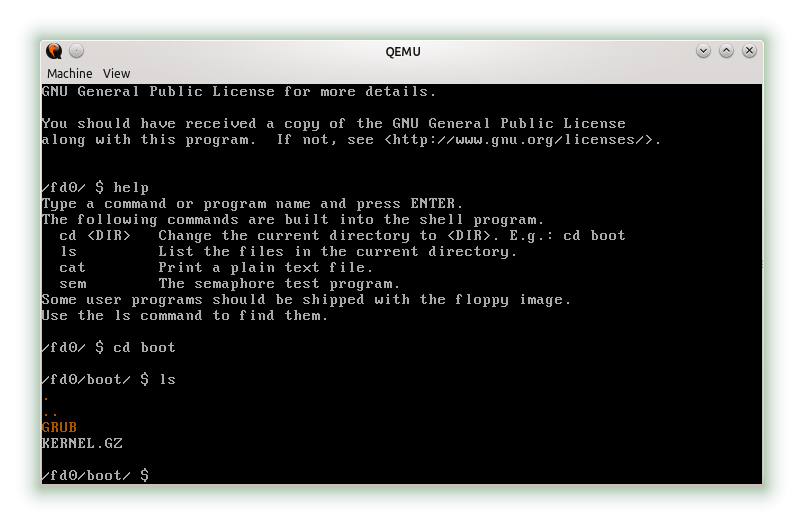
\includegraphics[scale=0.72]{1.png}
\end{figure}

在软盘根目录中包含了几个COM格式的用户程序。可以在根目录中通过\verb|ls|命令显示出来。

由于前一个实验中的信号量演示程序\verb|sem|需要共享内存,但AssignmentOS尚未实现\verb|shmX|系列
系统调用,因此该演示程序仍然只能内建到内核中,通过\verb|sem|命令运行。

\begin{figure}[htp!]
    \center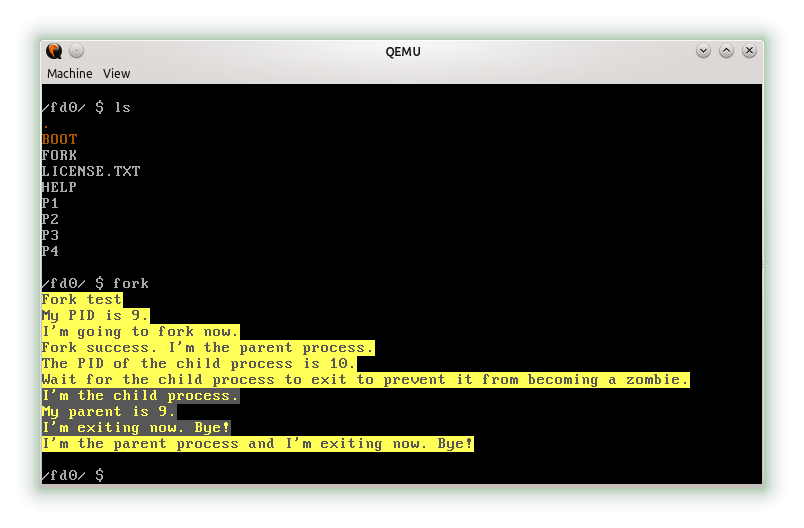
\includegraphics[scale=0.72]{2.png}
\end{figure}

\begin{figure}[htp!]
    \center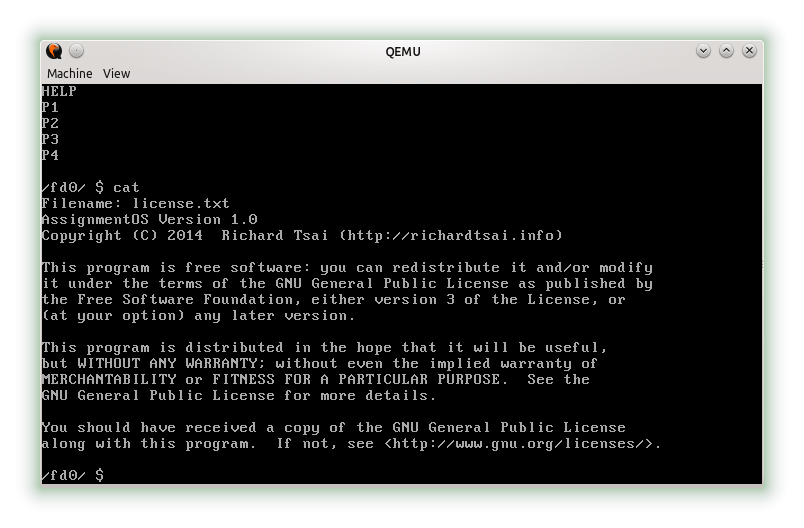
\includegraphics[scale=0.72]{3.png}
\end{figure}

\end{document}
